\documentclass[aspectratio=169,11pt]{beamer}

\usetheme{Madrid}
\usecolortheme{default}
\usefonttheme{professionalfonts}
\setbeamertemplate{navigation symbols}{}
\setbeamertemplate{footline}[frame number]

\usepackage{amsmath, amssymb, booktabs, graphicx}
\graphicspath{{../../assets/figures/}{assets/figures/}}

\title{Synthesis and Student Research Designs}
\subtitle{Labor II --- Week 13}
\author{Teaching deck draft}
\date{}

\begin{document}

\begin{frame}
  \titlepage
\end{frame}

\begin{frame}{Central question and why a synthesis week matters}
\begin{itemize}
    \item How do firm behavior, frictions, institutions, and shocks fit into one labor-market framework?
    \item Week 13 is not a loose recap. It turns the course sequence into a research toolkit.
    \item The capstone discipline is to name the mechanism, unit, observed margin, and equilibrium scope before making a big claim.
\end{itemize}
\end{frame}

\begin{frame}{Labor I to Labor II bridge}
\begin{itemize}
    \item Labor I centered workers: labor supply, human capital, mobility, inequality, discrimination, and household constraints.
    \item Labor II embedded those worker-side objects inside firms, wage-setting, search frictions, institutions, and major shocks.
    \item Together they form one field: worker choices filtered through market structure and institutional environments.
\end{itemize}
\end{frame}

\begin{frame}{Labor II architecture map}
\begin{center}
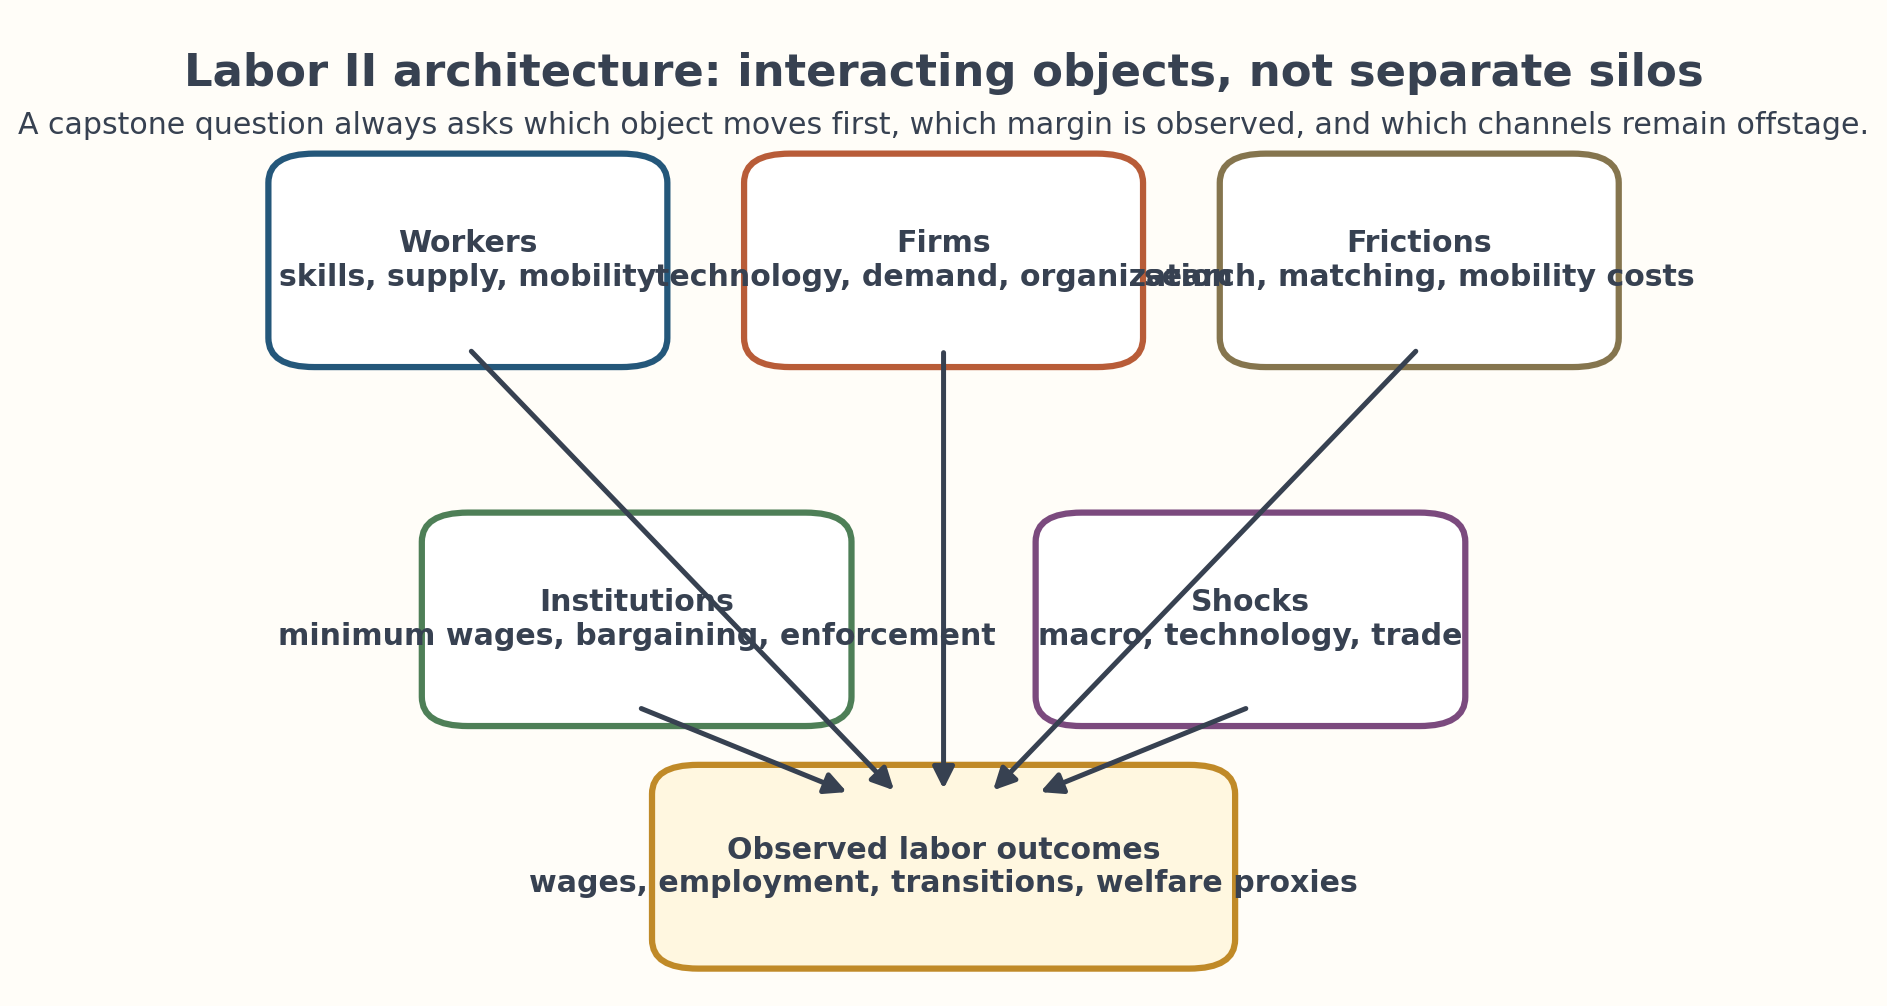
\includegraphics[height=0.73\textheight]{13-labor-ii-architecture-map.png}
\end{center}
\end{frame}

\begin{frame}{One architecture object for the semester}
\[
Y_{u,t+h} = \mathcal{G}\left(X^{\text{worker}}_{u,t},\; X^{\text{firm}}_{u,t},\; \mathcal{F}_{m,t},\; \mathcal{I}_{m,t},\; \mathcal{S}_{m,t:h}\right)
\]

\begin{itemize}
    \item The point is not that this is already a structural model.
    \item The point is to keep workers, firms, frictions, institutions, and shocks on the same conceptual page.
    \item The unit \(u\) changes with the question, and so does the claim the design can support.
\end{itemize}
\end{frame}

\begin{frame}{Choosing units of analysis}
\begin{itemize}
    \item Worker: earnings, employment, mobility, welfare distribution
    \item Firm or establishment: labor demand, organization, compliance, adoption
    \item Occupation or task: exposure, job content, classification
    \item Region or place: local incidence, spillovers, reallocation
    \item Market or regime: institutional coverage and equilibrium comparison
\end{itemize}
\end{frame}

\begin{frame}{Question -> mechanism -> unit -> design}
\begin{center}
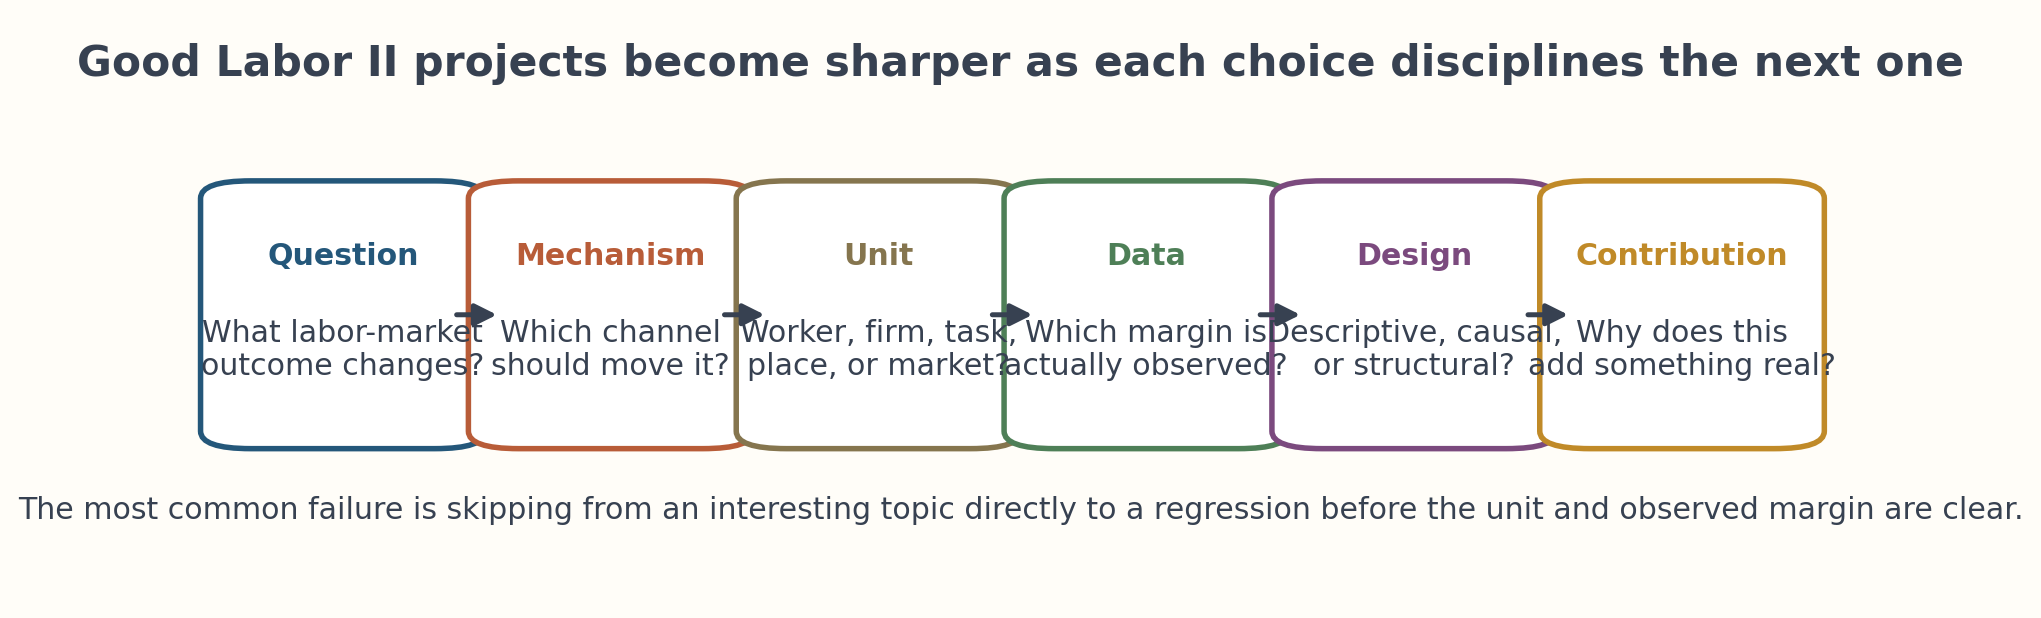
\includegraphics[width=0.96\textwidth]{13-question-mechanism-unit-design.png}
\end{center}
\end{frame}

\begin{frame}{Descriptive, reduced-form, and structural approaches}
\[
\Delta y_{u,t+h} = \beta D_{u,t} + X_{u,t}'\Gamma + \varepsilon_{u,t+h}
\]

\begin{itemize}
    \item Descriptive work is strongest when the field lacks a clean object or measurement frame.
    \item Reduced-form work is strongest when treatment, mechanism, and observed margin line up tightly.
    \item Structural work is necessary when the question itself is about equilibrium propagation, welfare, or policy counterfactuals.
\end{itemize}
\end{frame}

\begin{frame}{Comparative synthesis: wage-setting and labor market power}
\begin{itemize}
    \item Labor demand sets the value of labor to firms.
    \item Search, bargaining, and posting shape surplus division and wage dispersion.
    \item Monopsony turns mobility frictions into markdowns and firm labor-market power.
    \item Unions and wage regulation change voice, coverage, compression, and incidence.
\end{itemize}
\end{frame}

\begin{frame}{Comparative synthesis: regulation and institutions}
\begin{itemize}
    \item Ask four questions: which margin is targeted, who is covered, where do spillovers go, and what welfare object is implied?
    \item Minimum wages, bargaining systems, labor law, enforcement, and insurance are distinct institutional treatments.
    \item Coverage without enforcement is weak treatment; direct effects without spillovers are incomplete interpretation.
\end{itemize}
\end{frame}

\begin{frame}{Comparative synthesis: macro, technology, and trade adjustment}
\begin{itemize}
    \item Macro shocks: vacancies, unemployment, separations, wage cyclicality
    \item Technology shocks: tasks, adoption, learning, local reallocation
    \item Trade shocks: import exposure, offshoring, place incidence, long-run worker adjustment
    \item Across all three, short-run incidence and long-run welfare are different objects.
\end{itemize}
\end{frame}

\begin{frame}{Policies versus shocks}
\begin{center}
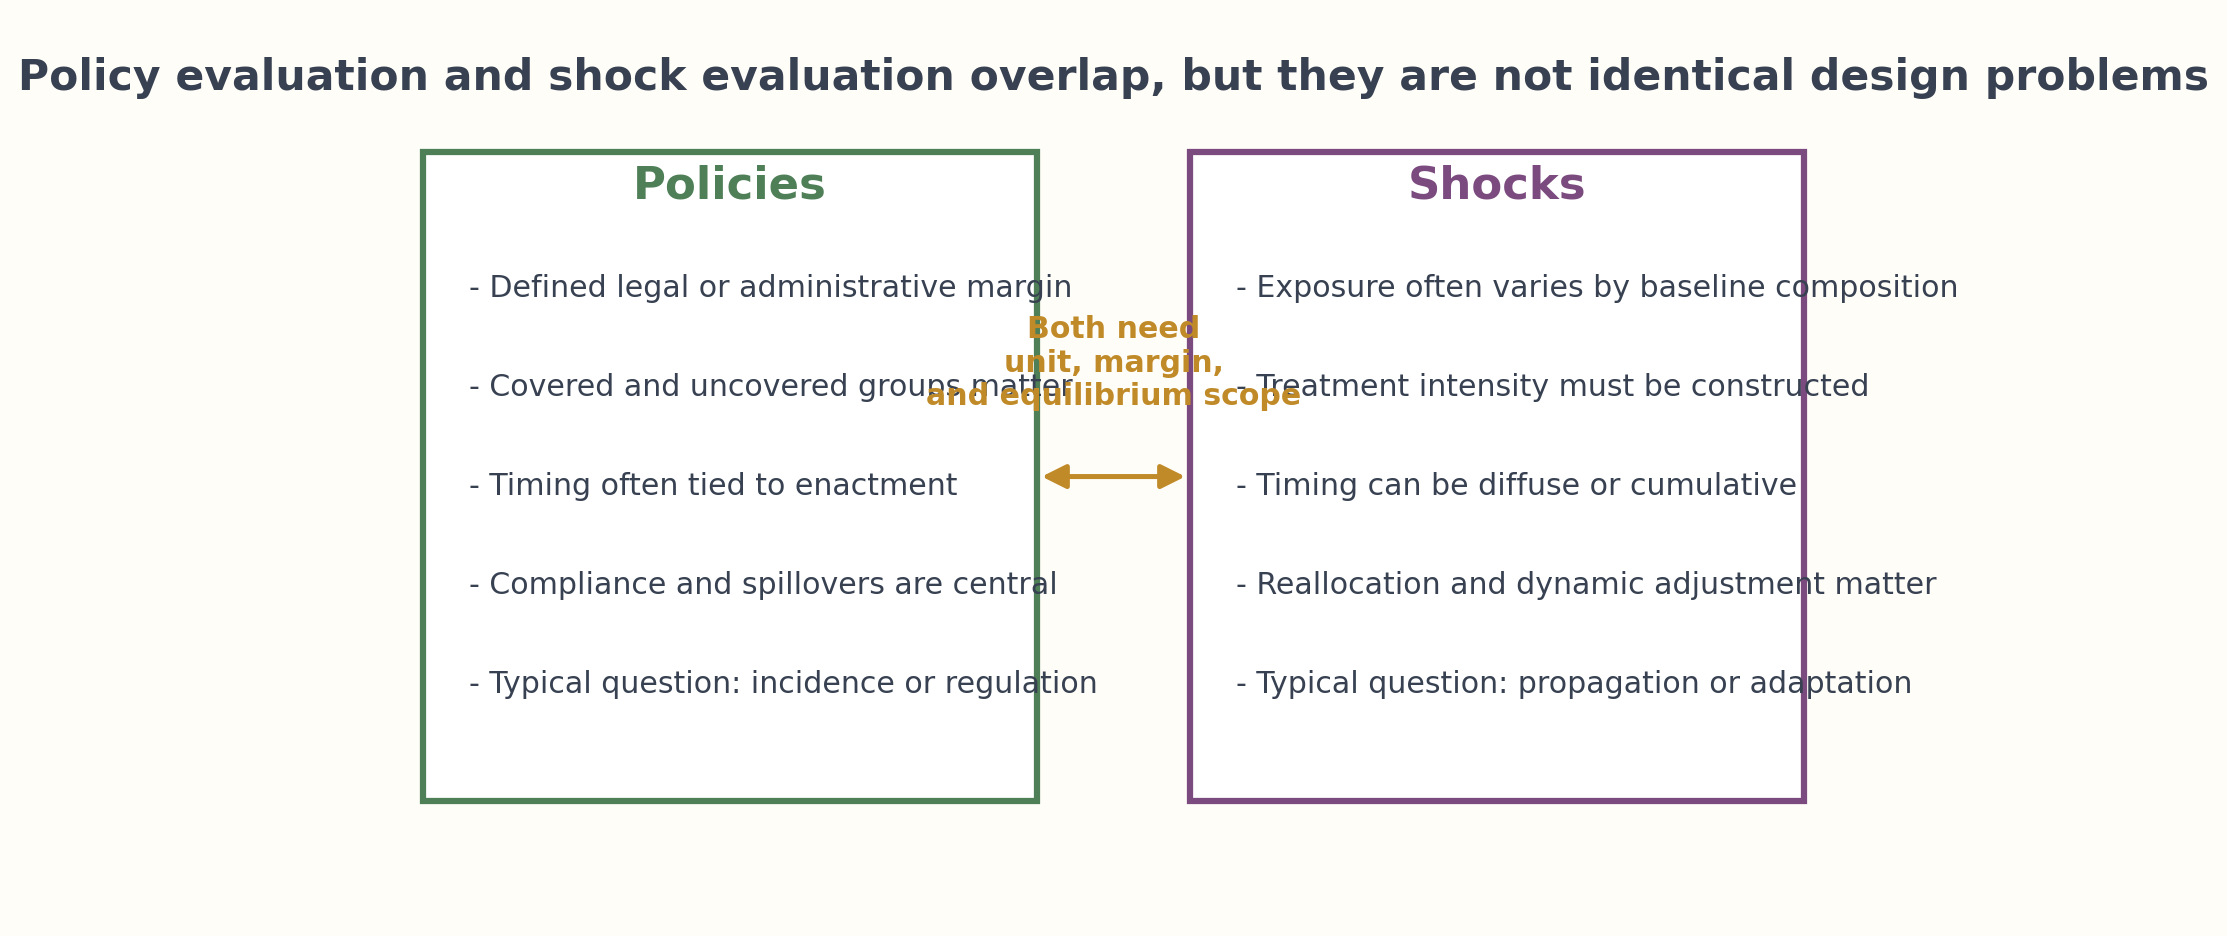
\includegraphics[height=0.73\textheight]{13-policy-vs-shock-comparison.png}
\end{center}
\end{frame}

\begin{frame}{Partial equilibrium versus equilibrium reasoning}
\[
\Delta W \neq \omega \cdot \beta
\]

\begin{itemize}
    \item A wage, employment, or transition coefficient is not automatically a welfare statement.
    \item Place effects do not automatically equal worker welfare effects.
    \item Short-run treatment effects do not automatically reveal long-run adjustment.
    \item Stronger claims require explicit spillover, incidence, and aggregation structure.
\end{itemize}
\end{frame}

\begin{frame}{How to build a research idea}
\begin{itemize}
    \item Question: what labor-market outcome needs explanation?
    \item Mechanism: through which disciplined channel?
    \item Unit: worker, firm, task, place, or market?
    \item Data: which margin is directly observed?
    \item Design: descriptive, reduced-form, or structural?
    \item Contribution: what does the project add beyond a re-description of an existing paper?
\end{itemize}
\end{frame}

\begin{frame}{Common failure modes}
\begin{center}
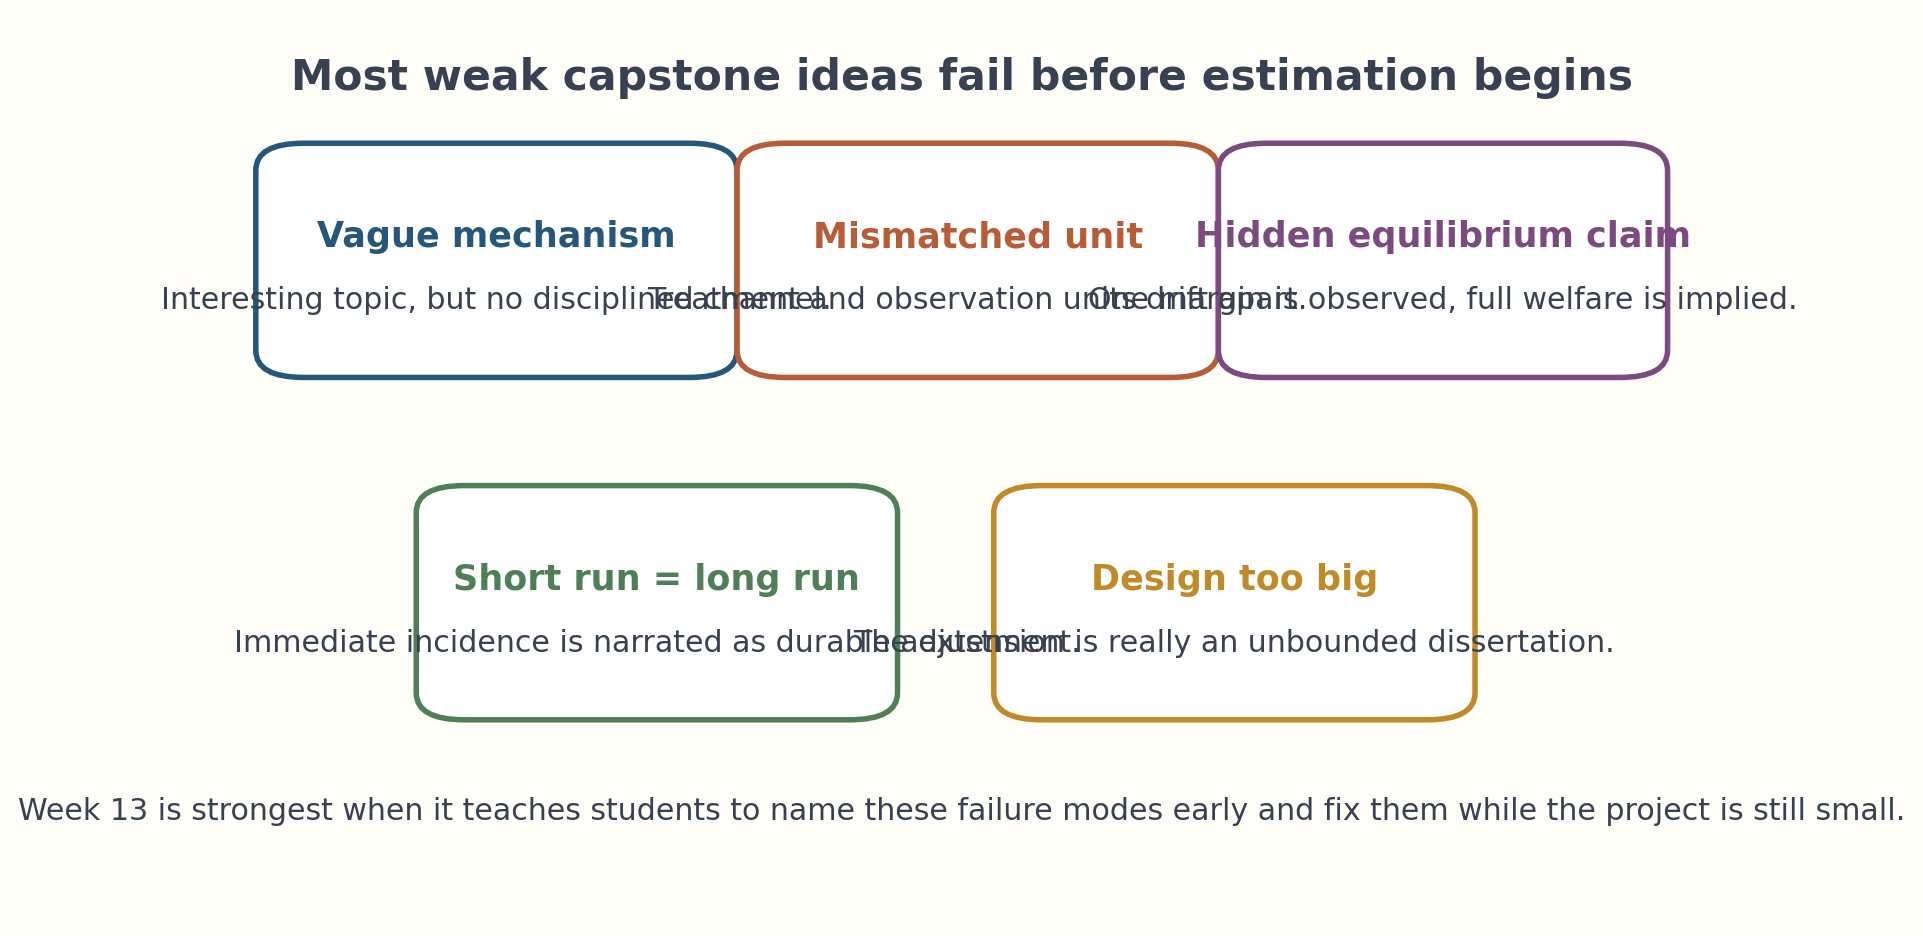
\includegraphics[height=0.72\textheight]{13-common-failure-modes.png}
\end{center}
\end{frame}

\begin{frame}{Frontier directions and bridge beyond Labor II}
\begin{center}
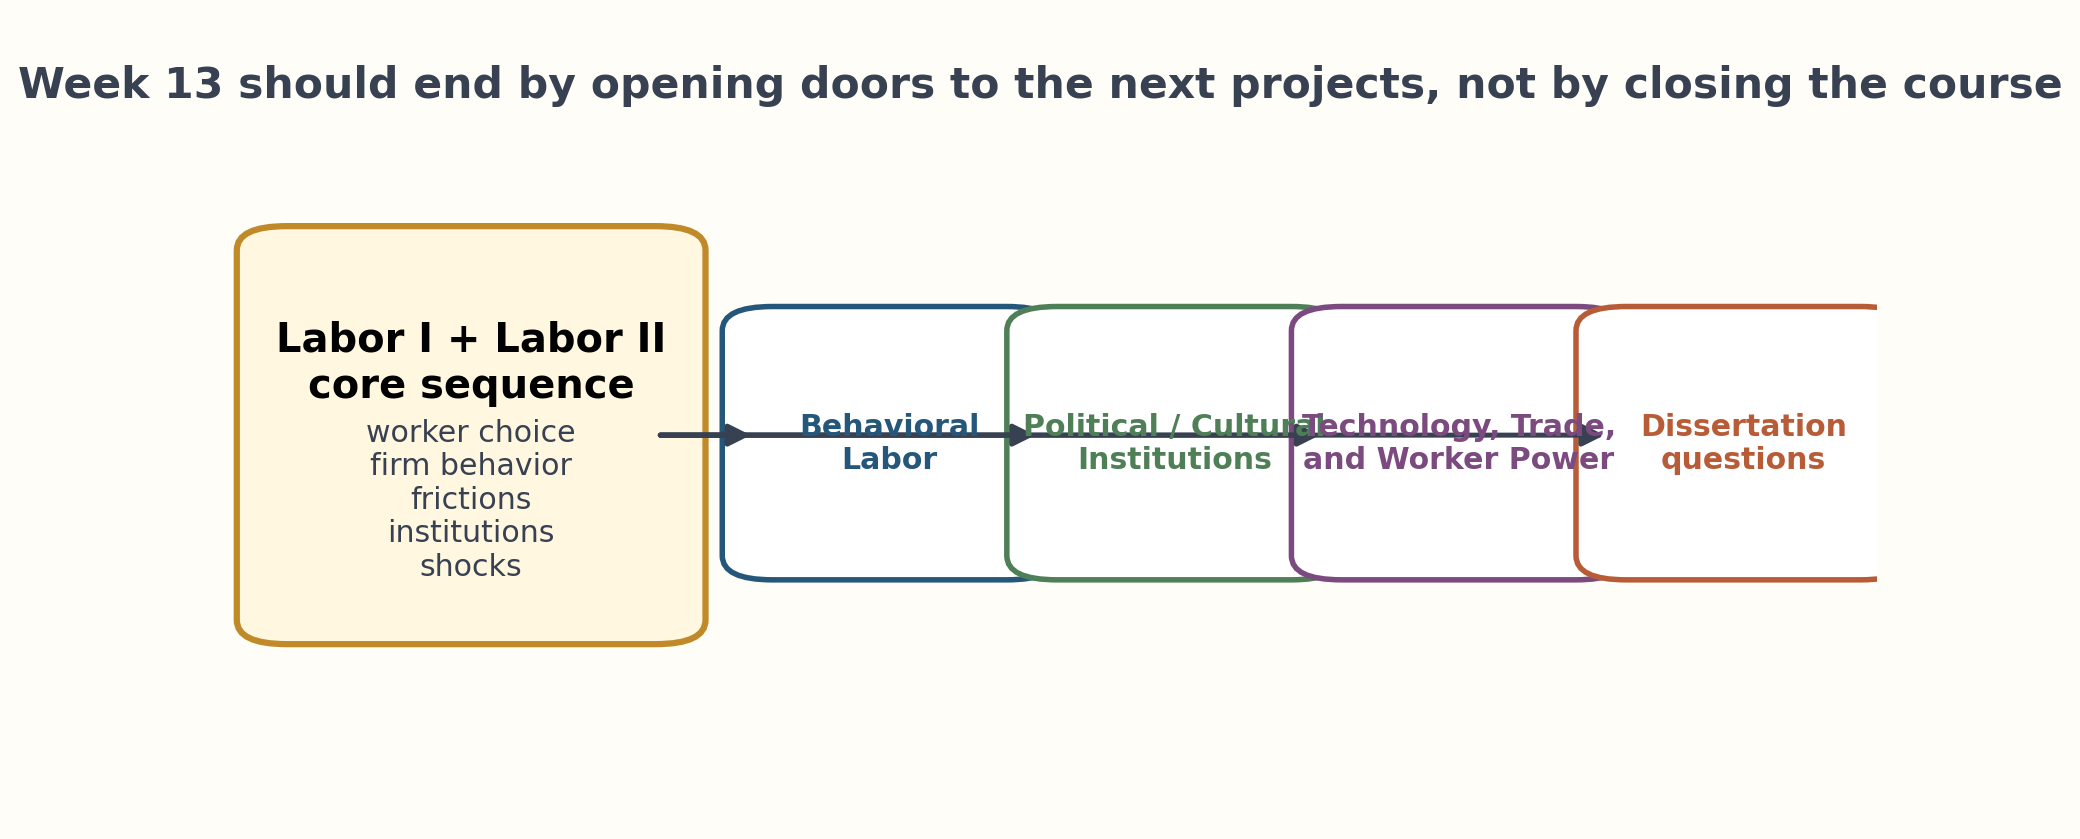
\includegraphics[width=0.94\textwidth]{13-frontier-and-dissertation-bridge.png}
\end{center}
\end{frame}

\begin{frame}{Bridge beyond the sequence}
\begin{itemize}
    \item Back to Labor I: worker heterogeneity, inequality, mobility, and human capital with stronger market-side discipline
    \item Forward to Behavioral Labor: search behavior, worker beliefs, and application technology under frictions
    \item Forward to institutions: bargaining, norms, enforcement, and political or cultural structure as labor-market objects
    \item Forward to dissertation work: bounded questions with clear units and honest equilibrium scope
\end{itemize}
\end{frame}

\begin{frame}{Takeaways}
\begin{itemize}
    \item Labor II works best as one architecture linking workers, firms, frictions, institutions, and shocks.
    \item Unit choice, observed margin, and equilibrium scope are core design choices, not afterthoughts.
    \item Descriptive, reduced-form, and structural approaches answer different questions and should not be ranked mechanically.
    \item The capstone goal is to turn a mechanism into a research design that is sharp, bounded, and useful.
\end{itemize}
\end{frame}

\appendix

\begin{frame}{Appendix: Week 13 lab bridge}
\begin{itemize}
    \item Diagnose: identify mechanism, treatment unit, observation unit, observed margin, and equilibrium concern.
    \item Compare: pair one anchor paper with a nearby design that changes the unit or treatment family.
    \item Design: produce a memo scaffold for a bounded extension rather than a vague final-project idea.
    \item The studio artifact is a disciplined starting point for field papers, workshops, or dissertation questions.
\end{itemize}
\end{frame}

\end{document}
